\clearpage

\subsection{Opaque with 1+1 Protection}\label{heuristic_Opaque_Protection}
\begin{tcolorbox}	
\begin{tabular}{p{2.75cm} p{0.2cm} p{10.5cm}} 	
\textbf{Student Name}  &:& Pedro Coelho    (March 01, 2018 - )\\
\textbf{Goal}          &:& Implement the heuristic model for the opaque transport mode with 1 plus 1 protection.
\end{tabular}
\end{tcolorbox}

\subsubsection{Model description}

The impact of failure in WDM (Wavelength Division Multiplexing) networks is caused by extremely high volume of traffic carried. In a high speed network like the WDM, a failure of a network element may cause failure of various optical channels that leads to large data and revenue losses, which can interrupt communication services.

In this protection scheme, the primary and backup path carry the traffic end-to-end, i.e., there is a need to have a backup path (the unaffected path) in case of a network failure. Then, the receiver will decide which one of the two incoming traffic it is going to pick, if the primary or the backup path.

Although it is the fastest protection scheme, it is also the most expensive, because it normally uses more than the double of the capacity for the primary path. This happens because the backup path is typically longer than the primary.

For this protection model, after the creation of the matrices and the network topology, it is necessary to apply the routing and grooming algorithms created. For the "Logical Topology" algorithm, the user must insert "Opaque" in the "logicalTopology" value and for the "Grooming" algorithm, the user must insert "yes" in the parameter value "protection".

At the end, the "Cost Report" algorithm will be applied to obtain the best CAPEX result for the network in question.

Firstly, in the opaque transport mode, the optical node cost is 0 because all the ports in the network are electrical. Consequently, to calculate the node cost it only has to be considered the electrical node cost.

\begin{itemize}
  \item Where $N_{OXC,n}$ = 0, \quad $\forall$ n.
  \item Where $N_{EXC,n}$ = 1, \quad $\forall$ n that process traffic.
\end{itemize}

Still referring to the electrical node cost, the number of long-reach ports of the electrical switch, i.e., the number of line ports of a node n is calculated by the equation \ref{EXC_pexc1_opaque_heuristic_protec}.

\begin{equation}
P_{exc,-1,n} = \sum_{j=1}^{N} w_{nj}
\label{EXC_pexc1_opaque_heuristic_protec}
\end{equation}

\begin{itemize}
\item Where {$w_{nj}$ is the number of optical channels between node $n$ and node $j$}.
\end{itemize}

\newpage
\vspace{11pt}
In addition, the number of short-reach ports of the electrical switch, i.e., the number of tributary ports with bit-rate c in a node n is calculated by the equation \ref{EXC_pexc2_opaque_heuristic_protec}.

\begin{equation}
P_{exc,c,n} = \sum_{d=1}^{N} D_{nd,c}
\label{EXC_pexc2_opaque_heuristic_protec}
\end{equation}

\begin{itemize}
  \item Where {$D_{nd,c}$ are the client demands between nodes $n$ and $d$ with bit rate $c$}.
\end{itemize}

\vspace{11pt}
In this case there is the following particularity:

\begin{itemize}
  \item When $n$=$j$, the value of client demands is always zero, i.e, $D_{nn,c}=0$.
\end{itemize}

\subsubsection{Result description}

It is already known all the necessary formulas to obtain the CAPEX value for the reference network \ref{Reference_Network_Topology}. As described in the subsection of the network traffic \ref{Reference_Network_Traffic}, it is necessary to obtain three different values of CAPEX for the low (0.5 Tbit/s), medium (5 Tbit/s) and high (10 Tbit/s) traffic. It is used a network software program called Net2Plan which can design the traffic matrices, create all the network topologies, simulate the algorithms into the network implemented in the programming software called Eclipse and analyze the results obtained.\\

\textbf{Low Traffic Scenario:}\\

In this scenario it has to take into account the traffic calculated in \ref{low_traffic_scenario}. In a first phase it will be shown the three topologies of the network, the first one already knew allowed physical topology, the second one allowed optical topology and finally the physical topology.\\

\textbf{0.5 Tbit/s}

\begin{figure}[H]
\centering
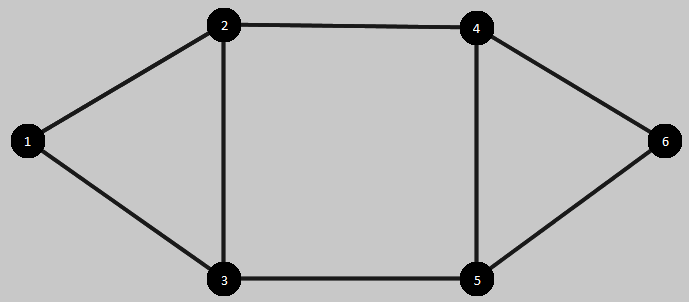
\includegraphics[width=13cm]{sdf/heuristic/figures/topological_design1}
\caption{Allowed physical topology of the reference network.}
\label{allowed_physical_surv_ref_low_heuristic}
\end{figure}

Following all the steps mentioned in the \ref{net2plan_guide}, applying the routing and grooming heuristic algorithms in the Net2Plan software and using all the data referring to this scenario, the obtained result can be consulted in the following table:

\begin{table}[H]
\centering
\begin{tabular}{|| c | c | c | c | c | c | c ||}
 \hline
 \multicolumn{7}{|| c ||}{CAPEX of the Network} \\
 \hline
 \hline
 \multicolumn{3}{|| c |}{ } & Quantity & Unit Price & Cost & Total \\
 \hline
 \multirow{3}{*}{Link Cost} & \multicolumn{2}{ c |}{OLTs} & 16 & 15 000 \euro & 240 000 \euro & \multirow{3}{*}{29 520 000 \euro} \\ \cline{2-6}
 & \multicolumn{2}{ c |}{100 Gb/s Transceivers} & 58 & 5 000 \euro/Gb/s & 29 000 000 \euro & \\ \cline{2-6}
 & \multicolumn{2}{ c |}{Amplifiers} & 70 & 4 000 \euro & 280 000 \euro & \\
 \hline
 \multirow{9}{*}{Node Cost} & \multirow{7}{*}{Electrical} & EXCs & 6 & 10 000 \euro & 60 000 \euro & \multirow{9}{*}{5 862 590 \euro} \\ \cline{3-6}
 & & ODU0 Ports & 60 & 8 \euro/Gb/s & 600 \euro & \\ \cline{3-6}
 & & ODU1 Ports & 50 & 6 \euro/Gb/s & 750 \euro & \\ \cline{3-6}
 & & ODU2 Ports & 16 & 3 \euro/Gb/s & 480 \euro & \\ \cline{3-6}
 & & ODU3 Ports & 6 & 1.5 \euro/Gb/s & 360 \euro & \\ \cline{3-6}
 & & ODU4 Ports & 4 & 1 \euro/Gb/s & 400 \euro & \\ \cline{3-6}
 & & Line Ports & 58 & 1 000 \euro/Gb/s & 5 800 000 \euro & \\ \cline{2-6}
 & \multirow{2}{*}{Optical} & OXCs & 0 & 20 000 \euro & 0 \euro & \\ \cline{3-6}
 & & Ports & 0 & 2 500 \euro/porto & 0 \euro & \\
 \hline
 \multicolumn{6}{|| c |}{Total Network Cost} & 35 382 590 \euro \\
\hline
\end{tabular}
\caption{Table with detailed description of CAPEX}
\label{scriptopaque_protec_ref_low_heuristic}
\end{table}

Through the formulas mentioned below it can be demonstrated how all the values of the quantity column were calculated.

\begin{equation*}
 OLTs: 2 \sum_{(i,j):i<j}L_{ij} \qquad \qquad
 Transceivers: 2 \sum_{(i,j):i<j}W_{ij} \qquad \qquad
 Amplifiers: \sum_{(i,j):i<j}N^R_{ij} L_{ij} \\
\end{equation*}
\begin{equation*}
 EXCs: \sum_n^N N_{EXC,n} \qquad
 ODU0: \sum_{(o,d)}^{N}D_{od,0} \qquad \qquad
 ODU1: \sum_{(o,d)}^{N}D_{od,1} \qquad
 ODU2: \sum_{(o,d)}^{N}D_{od,2}
\end{equation*}
\begin{equation*}
 ODU3: \sum_{(o,d)}^{N}D_{od,3} \qquad \qquad
 ODU4: \sum_{(o,d)}^{N}D_{od,4} \qquad \qquad
 Line: \sum_{(i,j)}^{N}W_{ij}
\end{equation*}

\vspace{13pt}
$OXCs: \sum_n^N N_{OXC,n}$ but as mentioned initially this result is always zero \\

$Ports$: does not exist for this case then it is equal to zero \\

\newpage
\textbf{Medium Traffic Scenario:}\\

In this scenario it has to take into account the traffic calculated in \ref{medium_traffic_scenario}. In a first phase it will be shown the three topologies of the network, the first one already knew allowed physical topology, the second one allowed optical topology and finally the physical topology.\\

\textbf{5 Tbit/s}

\begin{figure}[H]
\centering
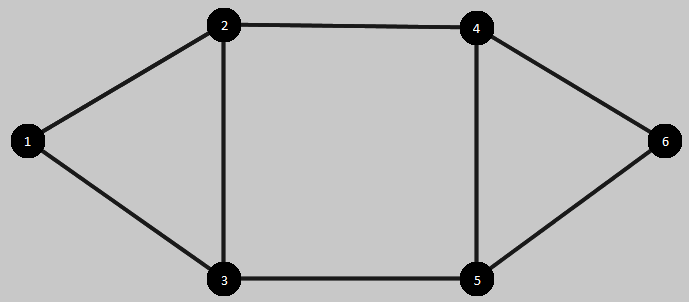
\includegraphics[width=13cm]{sdf/heuristic/figures/topological_design1}
\caption{Allowed physical topology of the reference network.}
\label{allowed_physical_surv_ref_low_heuristic}
\end{figure}

Following all the steps mentioned in the \ref{net2plan_guide}, applying the routing and grooming heuristic algorithms in the Net2Plan software and using all the data referring to this scenario, the obtained result can be consulted in the following table:

\begin{table}[H]
\centering
\begin{tabular}{|| c | c | c | c | c | c | c ||}
 \hline
 \multicolumn{7}{|| c ||}{CAPEX of the Network} \\
 \hline
 \hline
 \multicolumn{3}{|| c |}{ } & Quantity & Unit Price & Cost & Total \\
 \hline
 \multirow{3}{*}{Link Cost} & \multicolumn{2}{ c |}{OLTs} & 16 & 15 000 \euro & 240 000 \euro & \multirow{3}{*}{250 520 000 \euro} \\ \cline{2-6}
 & \multicolumn{2}{ c |}{100 Gb/s Transceivers} & 500 & 5 000 \euro/Gb/s & 250 000 000 \euro & \\ \cline{2-6}
 & \multicolumn{2}{ c |}{Amplifiers} & 70 & 4 000 \euro & 280 000 \euro & \\
 \hline
 \multirow{9}{*}{Node Cost} & \multirow{7}{*}{Electrical} & EXCs & 6 & 10 000 \euro & 60 000 \euro & \multirow{9}{*}{50 062 590 \euro} \\ \cline{3-6}
 & & ODU0 Ports & 60 & 8 \euro/Gb/s & 600 \euro & \\ \cline{3-6}
 & & ODU1 Ports & 50 & 6 \euro/Gb/s & 750 \euro & \\ \cline{3-6}
 & & ODU2 Ports & 16 & 3 \euro/Gb/s & 480 \euro & \\ \cline{3-6}
 & & ODU3 Ports & 6 & 1.5 \euro/Gb/s & 360 \euro & \\ \cline{3-6}
 & & ODU4 Ports & 4 & 1 \euro/Gb/s & 400 \euro & \\ \cline{3-6}
 & & Line Ports & 500 & 1 000 \euro/Gb/s & 50 000 000 \euro & \\ \cline{2-6}
 & \multirow{2}{*}{Optical} & OXCs & 0 & 20 000 \euro & 0 \euro & \\ \cline{3-6}
 & & Ports & 0 & 2 500 \euro/porto & 0 \euro & \\
 \hline
 \multicolumn{6}{|| c |}{Total Network Cost} & 300 582 590 \euro \\
\hline
\end{tabular}
\caption{Table with detailed description of CAPEX}
\label{scriptopaque_protec_ref_medium_heuristic}
\end{table}

Through the formulas mentioned below it can be demonstrated how all the values of the quantity column were calculated.

\begin{equation*}
 OLTs: 2 \sum_{(i,j):i<j}L_{ij} \qquad \qquad
 Transceivers: 2 \sum_{(i,j):i<j}W_{ij} \qquad \qquad
 Amplifiers: \sum_{(i,j):i<j}N^R_{ij} L_{ij} \\
\end{equation*}
\begin{equation*}
 EXCs: \sum_n^N N_{EXC,n} \qquad
 ODU0: \sum_{(o,d)}^{N}D_{od,0} \qquad \qquad
 ODU1: \sum_{(o,d)}^{N}D_{od,1} \qquad
 ODU2: \sum_{(o,d)}^{N}D_{od,2}
\end{equation*}
\begin{equation*}
 ODU3: \sum_{(o,d)}^{N}D_{od,3} \qquad \qquad
 ODU4: \sum_{(o,d)}^{N}D_{od,4} \qquad \qquad
 Line: \sum_{(i,j)}^{N}W_{ij}
\end{equation*}

\vspace{13pt}
$OXCs: \sum_n^N N_{OXC,n}$ but as mentioned initially this result is always zero \\

$Ports$: does not exist for this case then it is equal to zero \\

\textbf{High Traffic Scenario:}\\

In this scenario it has to take into account the traffic calculated in \ref{high_traffic_scenario}. In a first phase it will be shown the three topologies of the network, the first one already knew allowed physical topology, the second one allowed optical topology and finally the physical topology.\\

\textbf{10 Tbit/s}

\begin{figure}[H]
\centering
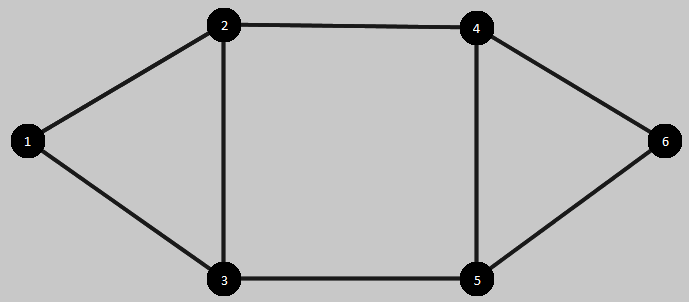
\includegraphics[width=13cm]{sdf/heuristic/figures/topological_design1}
\caption{Allowed physical topology of the reference network.}
\label{allowed_physical_surv_ref_low_heuristic}
\end{figure}

Following all the steps mentioned in the \ref{net2plan_guide}, applying the routing and grooming heuristic algorithms in the Net2Plan software and using all the data referring to this scenario, the obtained result can be consulted in the following table:

\begin{table}[H]
\centering
\begin{tabular}{|| c | c | c | c | c | c | c ||}
 \hline
 \multicolumn{7}{|| c ||}{CAPEX of the Network} \\
 \hline
 \hline
 \multicolumn{3}{|| c |}{ } & Quantity & Unit Price & Cost & Total \\
 \hline
 \multirow{3}{*}{Link Cost} & \multicolumn{2}{ c |}{OLTs} & 16 & 15 000 \euro & 240 000 \euro & \multirow{3}{*}{497 520 000 \euro} \\ \cline{2-6}
 & \multicolumn{2}{ c |}{100 Gb/s Transceivers} & 994 & 5 000 \euro/Gb/s & 497 000 000 \euro & \\ \cline{2-6}
 & \multicolumn{2}{ c |}{Amplifiers} & 70 & 4 000 \euro & 280 000 \euro & \\
 \hline
 \multirow{9}{*}{Node Cost} & \multirow{7}{*}{Electrical} & EXCs & 6 & 10 000 \euro & 60 000 \euro & \multirow{9}{*}{99 462 590 \euro} \\ \cline{3-6}
 & & ODU0 Ports & 60 & 8 \euro/Gb/s & 600 \euro & \\ \cline{3-6}
 & & ODU1 Ports & 50 & 6 \euro/Gb/s & 750 \euro & \\ \cline{3-6}
 & & ODU2 Ports & 16 & 3 \euro/Gb/s & 480 \euro & \\ \cline{3-6}
 & & ODU3 Ports & 6 & 1.5 \euro/Gb/s & 360 \euro & \\ \cline{3-6}
 & & ODU4 Ports & 4 & 1 \euro/Gb/s & 400 \euro & \\ \cline{3-6}
 & & Line Ports & 994 & 1 000 \euro/Gb/s & 99 400 000 \euro & \\ \cline{2-6}
 & \multirow{2}{*}{Optical} & OXCs & 0 & 20 000 \euro & 0 \euro & \\ \cline{3-6}
 & & Ports & 0 & 2 500 \euro/porto & 0 \euro & \\
 \hline
 \multicolumn{6}{|| c |}{Total Network Cost} & 596 982 590 \euro \\
\hline
\end{tabular}
\caption{Table with detailed description of CAPEX}
\label{scriptopaque_protec_ref_high_heuristic}
\end{table}

Through the formulas mentioned below it can be demonstrated how all the values of the quantity column were calculated.

\begin{equation*}
 OLTs: 2 \sum_{(i,j):i<j}L_{ij} \qquad \qquad
 Transceivers: 2 \sum_{(i,j):i<j}W_{ij} \qquad \qquad
 Amplifiers: \sum_{(i,j):i<j}N^R_{ij} L_{ij} \\
\end{equation*}
\begin{equation*}
 EXCs: \sum_n^N N_{EXC,n} \qquad
 ODU0: \sum_{(o,d)}^{N}D_{od,0} \qquad \qquad
 ODU1: \sum_{(o,d)}^{N}D_{od,1} \qquad
 ODU2: \sum_{(o,d)}^{N}D_{od,2}
\end{equation*}
\begin{equation*}
 ODU3: \sum_{(o,d)}^{N}D_{od,3} \qquad \qquad
 ODU4: \sum_{(o,d)}^{N}D_{od,4} \qquad \qquad
 Line: \sum_{(i,j)}^{N}W_{ij}
\end{equation*}

\vspace{13pt}
$OXCs: \sum_n^N N_{OXC,n}$ but as mentioned initially this result is always zero \\

$Ports$: does not exist for this case then it is equal to zero \\
